\documentclass[../main.tex]{subfiles}
\begin{document}
\section{神经网络}

\subsection{感知器}
\begin{enumerate}
    \item \textbf{一般形式：}感知器以一个实数值向量作为输入，计算这些输入的线性组合，如果结果大于某个阈值，就输出1，否则输出-1\footnote{可以把感知器看作是n维实例空间（即点空间）中的超平面决策面，对于超平面一侧的实例，感知器输出1，对于另一侧的实例，输出-1；可以被某个超平面分割的样例集合，称为线性可分样例集合}。
    \[
    o(x_1,\ldots,x_n)=
    \begin{cases}
    1, & w_0 + w_1x_1 + \cdots + w_nx_n > 0 \\
    -1, & \text{otherwise}
    \end{cases}
    \]
    其中每个 $w_i$ 是一个实数常量，也叫做权值，用来决定输入 $x_i$ 对感知器输出的贡献率。特别地，$w_0$ 是阈值。
    \item \textbf{简化形式（2种）：}
    \begin{enumerate}
        \item
        \[
        \sum_{i=0}^{n} w_i x_i > 0
        \]
        \item
        \[
        \vec{w}\cdot\vec{x} > 0
        \]
    \end{enumerate}
    \item \textbf{感知器函数：}
    \[
        o(\vec{x}) = \operatorname{sgn}(\vec{w}\cdot\vec{x})
    \]
    其中
    \[
        \operatorname{sgn}(y)=
        \begin{cases}
            1, & y > 0 \\
            -1, & \text{otherwise}
        \end{cases}
    \]
    \item \textbf{表征能力：}
    \begin{itemize}
        \item 感知器可以表示所有的\textbf{原子}布尔函数：与、或、与非、或非；
        \item 一些布尔函数无法用单一的感知器表示，例如异或；
        \item 因为所有的布尔函数都可表示为基于原子函数的互连单元的某个网络，因此，感知器网络可以表示所有的布尔函数。事实上，只需要两层深度的网络，比如表示析取范式.
        \item 要把一个AND感知器的输入求反只要简单地改变相应输入权的符号。
    \end{itemize}
    \item \textbf{训练法则：}
    \begin{enumerate}
        \item \textbf{感知器法则}：从随机的权值开始，反复应用这个感知器到每个训练样例，只要它误分类样例就修改感知器的权值，重复这个过程，直到感知器正确分类所有的训练样例；
        \[
        w_i \leftarrow w_i + \Delta w_i
        \]
        \[
        \Delta w_i = \eta (t - o)x_i
        \]
        \begin{itemize}
            \item \textbf{收敛的前提条件：}训练样例线性可分\footnote{存在一条直线（二维）、一个平面（三维）或更一般地一个超平面（高维），能够把所有正例和反例完全分开。}，且且使用了充分小的$\eta$。
        \end{itemize}
        \item \textbf{delta法则}：使用梯度下降来搜索可能的权向量的假设空间，以找到最佳拟合训练样例的权向量。又称增量法则、LMS 法则、Adaline 法则、Widrow-Hoff 法则\footnote{delta 法则可用于训练非阈值线性单元，也可用于训练有阈值的感知器单元；delta 法则优化的是线性单元的连续输出误差；阈值分类是否正确只取决于输出符号，因此连续误差变小通常有助于分类，但并不保证分类误差也最小。}。
        \begin{itemize}
            \item \textbf{基本更新式：}
            \[
                \vec{w}\leftarrow \vec{w}+\Delta\vec{w}
            \]
            \[
                \Delta\vec{w}=-\eta \nabla E(\vec{w})
            \]
            \item \textbf{无阈值线性单元：}可将 delta 训练法则理解为训练一个无阈值的感知器，其输出为
            \[
                o(\vec{x})=\vec{w}\cdot\vec{x}
            \]
            \item \textbf{训练误差：}指定误差函数
            \[
                E(\vec{w})=\frac{1}{2}\sum_{d\in D}(t_d-o_d)^2
            \]
            其中 $t_d$ 为目标输出，$o_d$ 为实际输出\footnote{在一定条件下，使 $E$ 最小化的假设就是 $H$ 中最可能的假设。}。

            \item \textbf{梯度下降算法：}
            \begin{itemize}
                \item 选取一个初始的随机权向量；
                \item 应用线性单元到所有训练样例，根据公式计算每个权值的更新值；
                \item 在终止条件满足前重复上述过程。
            \end{itemize}

            \item \textbf{线性单元的梯度下降训练过程：}
            \begin{itemize}
                \item 初始化每个 $w_i$ 为某个小的随机值；
                \item 遇到终止条件之前，重复以下操作：
                \begin{itemize}
                    \item 初始化每个 $\Delta w_i$ 为 0；
                    \item 对于训练集中的每个训练样例 $\langle \vec{x}, t \rangle$：
                    \begin{itemize}
                        \item 将实例 $\vec{x}$ 输入单元，计算输出 $o$；
                        \item 对每个权增量作更新：
                        \[
                            \Delta w_i \leftarrow \Delta w_i + \eta (t-o)x_i
                        \]
                    \end{itemize}
                    \item 对每个权值作更新：
                    \[
                        w_i \leftarrow w_i + \Delta w_i
                    \]
                \end{itemize}
            \end{itemize}

            \item \textbf{梯度下降的随机近似：}
            \begin{itemize}
                \item 梯度下降适用于假设空间包含连续参数化的假设，且误差对这些参数可微的情形；但收敛过程可能较慢，且若误差曲面存在多个局部极小值，则不能保证找到全局最小值；
                \item 随机梯度下降（或增量梯度下降，SGD）\footnote{它可看作对真实梯度下降的一种合理近似；当学习速率足够小时，可以任意程度接近真正的梯度下降；与标准梯度下降相比，随机梯度下降每次更新只考查一个样例，计算量更小，并且有时可能避免陷入某些局部极小值。}用单个样本（或很小一批样本）算出来的更新方向，去近似整个训练集上的真实梯度\footnote{使用随机的梯度下降而不是真正的梯度下降。}：
                \[
                    \Delta w_i \leftarrow \eta (t-o)x_i,\qquad
                    w_i \leftarrow w_i+\Delta w_i
                \]
            \end{itemize}
        \end{itemize}
        \item \textbf{线性规划：}解线性不等式方程组的一种通用的有效方法，仅当训练样例线性可分时有解，无法扩展到训练多层网络，而delta法则可以很容易扩展到多层网络。
    \end{enumerate}
\end{enumerate}
\begin{table}[H]
    \centering
    \caption{感知器法则与 delta 法则的对比}
    \label{tab:perceptron-delta-compare}
    \begin{tabular}{p{3.2cm} p{5.6cm} p{5.6cm}}
        \toprule
        \textbf{对比项} & \textbf{感知器法则} & \textbf{delta 法则} \\
        \midrule
        权值更新依据 &
        根据阈值化的感知器输出的误差更新权值 &
        根据输入的非阈值化线性组合的误差来更新权值 \\
        \addlinespace
        收敛结果 &
        经过有限次的迭代收敛到一个能理想分类训练数据的假设 &
        可能经过极长的时间，渐近收敛到最小误差假设 \\
        \addlinespace
        收敛条件 &
        条件是训练样例线性可分 &
        无需训练样例是否线性可分 \\
        \bottomrule
    \end{tabular}
\end{table}

\subsection{非线性单元}
\begin{enumerate}
    \begin{figure}[H]
        \centering
        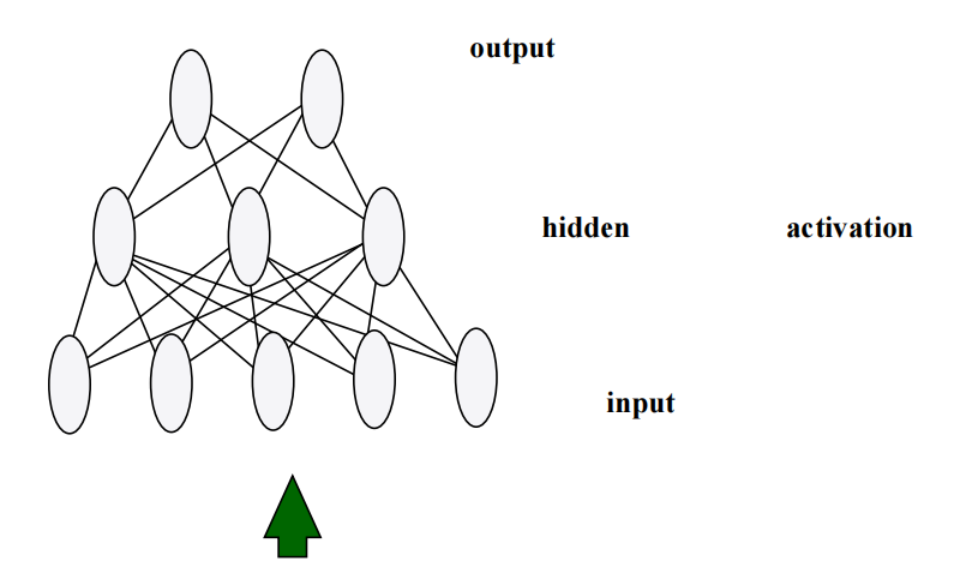
\includegraphics[width=0.5\linewidth]{images/multi_layer_net.png}
        \caption{典型的多层网络}
        \label{fig:placeholder}
    \end{figure}
    \item \textbf{多层网络}：络能够表示种类繁多的非线性曲面，由单元来连接，要求该单元：
    \begin{itemize}
        \item 输出是输入的非线性函数
        \item 输出是输入的可微函数
    \end{itemize}
    \item \textbf{sigmoid函数}：$o = \sigma \left( {\overrightarrow{w} \cdot  \overrightarrow{x}}\right)$，其中 $\sigma \left( y\right)  = \frac{1}{1 + {e}^{-y}}$
    \begin{itemize}
        \item 输出范围是0到1
        \item 单调递增
        \item 导数很容易用函数本身表示
    \end{itemize}
\end{enumerate}
\subsection{反向传播算法}
\begin{enumerate}
    \item \textbf{概念}：用来学习多层网络的权值，采用梯度下降方法试图最小化网络输出值和目标值之间的误差平方\footnote{它似乎默认损失函数就是 MSE，就这样吧，懒得管了。这里不整理太多了，如果确实有不了解反向传播算法的同学，推荐看 3Blue1Brown 的视频：\href{https://www.bilibili.com/video/BV16x411V7Qg/?spm_id_from=333.337.search-card.all.click&vd_source=5deca47094767260f853b759a625a68f}{B 站链接}}。
    \item \textbf{梯度下降更新法则与delta法则：}
    \begin{itemize}
        \item 同：依照以下三者来更新每一个权
        \begin{itemize}
            \item 学习速率 $\eta$
            \item 该权值涉及的输入值 ${\mathrm{x}}_{\mathrm{{ji}}}$
            \item 该单元的输出误差 $\delta$
        \end{itemize}
        \item 异：delta法则中的误差项被替换成一个更复杂的误差项 ${\delta }_{\mathrm{j}}$
    \end{itemize}
    \item \textbf{增加冲量项：}下面的第二项被称为冲量项\footnote{冲量有时会使这个球滚过误差曲面的局部极小值或平坦区域，也具有在梯度不变的区域逐渐增大搜索步长的效果,从而加快收敛。}
    $> \Delta {w}_{ji}\left( n\right)  = \eta {\delta }_{j}{x}_{ji} + {\alpha \Delta }{w}_{ji}\left( {n - 1}\right)$
    \item \textbf{推广性：}算法可以简单地推广到任意深度的前馈网络
    {\small\kaishu
    \begin{itemize}
     \item 第 $m$ 层的单元 $r$ 的 $\delta_r$ 值可由更深的第 $m+1$ 层的 $\delta$ 值按下式计算：
        \[
            \delta_r = o_r(1-o_r)\sum_{s\in \text{第 }m+1\text{ 层}} w_{sr}\delta_s
        \]
        其中：
        \begin{itemize}
            \item $\delta_r$ 表示第 $m$ 层单元 $r$ 的误差项；
            \item $o_r$ 表示单元 $r$ 的输出；
            \item $s$ 表示第 $m+1$ 层中与单元 $r$ 直接相连的单元；
            \item $w_{sr}$ 表示从单元 $r$ 到单元 $s$ 的连接权值；
            \item $\delta_s$ 表示下一层单元 $s$ 的误差项。
        \end{itemize}
    \end{itemize}
    }
\end{enumerate}
\subsection{前馈网络的表征能力}
\begin{enumerate}
    \item \textbf{布尔函数}：任何布尔函数可以被具有\textbf{两层}单元的网络准确表示，尽管在最坏情况下所需隐层单元的数量随着网络输入数量的增加成指数级增长。
    \item \textbf{连续函数}：每个有界的连续函数可以由一个\textbf{两层}的网络以任意小的误差\textbf{逼近}。这个结论适用于在隐藏层使用sigmoid单元、在输出层使用（非阈值）线性单元的网络。所需的隐层单元数量依赖于要逼近的函数。
    \item \textbf{任意函数}：任任意函数可以被一个有\textbf{三层}单元的网络以任意精度\textbf{逼近}。两个隐藏层使用sigmoid单元，输出层使用线性单元，每层所需单元数不确定。
\end{enumerate}

\subsection{假设空间搜索的本质特征}
\begin{enumerate}
    \item \textbf{假设空间搜索和归纳偏置：}
    {\small\kaishu
    \begin{itemize}
        \item 反向传播算法的假设空间是n个网络权值形成的n维欧氏空间。这个空间是连续的，与决策树学习和其它基于离散表示的方法的假设空间不同。
        \item 假设空间的连续性以及误差E关于假设的连续参数可微，导致了一个定义良好的误差梯度，为最佳假设的搜索提供了一个非常有用的结构。
        \item 精确地刻画出反向传播学习的归纳偏置是有难度的，它依赖于梯度下降搜索和权空间覆盖可表征函数空间的方式的相互作用性。
        \item 把这一偏置粗略地刻画为在数据点之间平滑插值。如果给定两个正例，它们之间没有反例，反向传播算法会倾向于把这两点之间的点也标记为正例。
    \end{itemize}
    }
    \item \textbf{隐藏层表示：}
    {\small\kaishu
    \begin{itemize}
        \item 反向传播算法的一个迷人特性是：它能够在网络内部的隐藏层发现有用的中间表示。
        \item 多层网络在隐藏层自动发现有用表示的能力是ANN学习的一个关键特性。允许学习器创造出设计者没有明确引入的特征。
        \item 网络中使用的单元层越多，就可以创造出越复杂的特征。
    \end{itemize}
    }
\end{enumerate}
\subsection{泛化、过拟合与停止判据}
\begin{enumerate}
    \item \textbf{权值更新算法的终止条件：}对训练样例的误差降低至某个预先定义的阈值之下？不好，因为反向传播容易过拟合
    \item \textbf{泛化精度：}网络拟合训练数据外的实例的精度
    \begin{figure}[H]
        \centering
        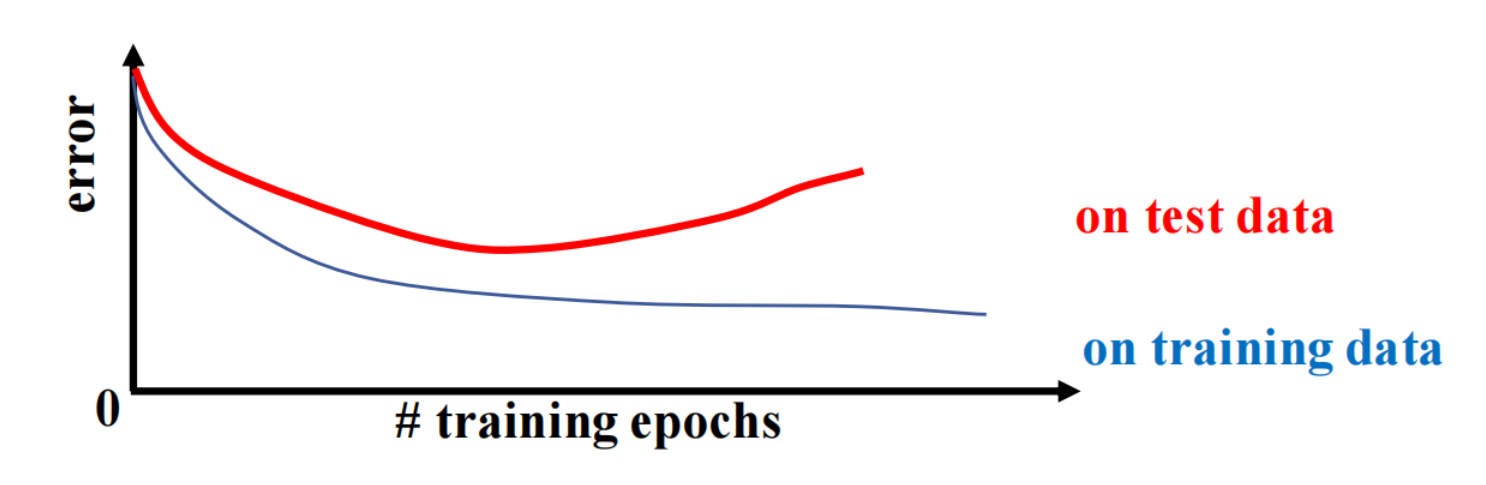
\includegraphics[width=0.75\linewidth]{images/guonihe.png}
        \caption{过拟合示例}
        \label{fig:placeholder}
    \end{figure}
    \item \textbf{为什么过拟合发生在迭代后期而不是早期？}
    
    {\small\kaishu
    设想网络的权值是被初始化为小随机值的，使用这些几乎一样的权值仅能描述非常平滑的决策面；随着训练的进行，一些权值开始增长，以降低在训练数据上的误差，同时学习到的决策面的复杂度也在增加；如果权值调整迭代次数足够多，反向传播算法可能会产生过度复杂的决策面，拟合了训练数据中的噪声和训练样例中没有代表性的特征。
    }
    \item \textbf{过拟合的解决办法：}权重衰减、验证数据、k-fold交叉验证\footnote{把训练样例分成k份，然后进行k次交叉验证过程，每次使用不同的一份作为验证集合，其余k-1份合并作为训练集合。每个样例会在一次实验中被用作验证样例，在k-1次实验中被用作训练样例；每次实验中，使用上面讨论的交叉验证过程来决定在验证集合上取得最佳性能的迭代次数，然后计算这些迭代次数的均值。}、减少隐层单元\footnote{应用交叉验证方法确定隐层单元数}、权值共享\footnote{把与不同单元或输入相关联的权“捆绑在一起”，强迫不同的网络权值取一致的值，通常是为了实施人类设计者事先知道的某个约束。首先在共享权值的每个单元分别更新各个权值，然后取这些权值的平均，再用这个平均值替换每个需要共享的权值}。


\subsection{其他ANN学习算法}
\begin{enumerate}
    \item \textbf{误差函数的改进：}权衰减、导数信息、交叉熵、权值共享
    \item \textbf{其它误差最小化过程：}线搜索、共轭梯度
    \item \textbf{递归网络：}时间展开、反向传播变体、时序建模
    \item \textbf{动态调整网络结构：}增长网络、级联相关、网络修剪
\end{enumerate}

\end{enumerate}
\end{document}